% !TeX document-id = {31322199-07d0-4e7b-ac39-8f4bff032313}
% !TeX root = workshop-codemash-2023.tex
% !TeX TXS-program:compile = txs:///pdflatex/[--shell-escape]
% !TeX encoding = UTF-8
% !TeX spellcheck = en_US
% https://orcid.org/0000-0003-4586-8500
% session details: https://www.codemash.org/session-details/?id=375030

% Other possible values are: 1610, 149, 54, 43 and 32.
% By default, it is to 128mm by 96mm(4:3)
\documentclass[aspectratio=169]{beamer} 
%\setbeamertemplate{headline navigation symbols}{}         % no navigation symbols
\usetheme{Warsaw}
\usecolortheme{seahorse}
\usepackage[absolute,overlay]{textpos} % Text positioning


%Information to be included in the title page:
\title{Build a Serverless Github Bot in GCP}
\subtitle{}
\author{Franklin Diaz}
\institute{DE:AD:10:C5}
\date{Tuesday January 10, 2023}

\begin{document}

%%% Title Slide %%%
\frame{\titlepage}


%\begin{frame}
%        \frametitle{Table of Contents}
%        \tableofcontents
%\end{frame}

% you can uncomment one of these for the whole doc, or add at the start of each section as desired                                                                            
\usebackgroundtemplate{
\includegraphics[width=\paperwidth]{../images/field.jpg}}
%\usebackgroundtemplate{
\includegraphics[width=\paperwidth]{../images/landscape.jpg}}
%\usebackgroundtemplate{
\includegraphics[width=\paperwidth]{../images/tree.jpg}}

\begin{frame}
	\frametitle{Overview: Usage}
	The big picture for operation.
	\vspace{2mm}
	
	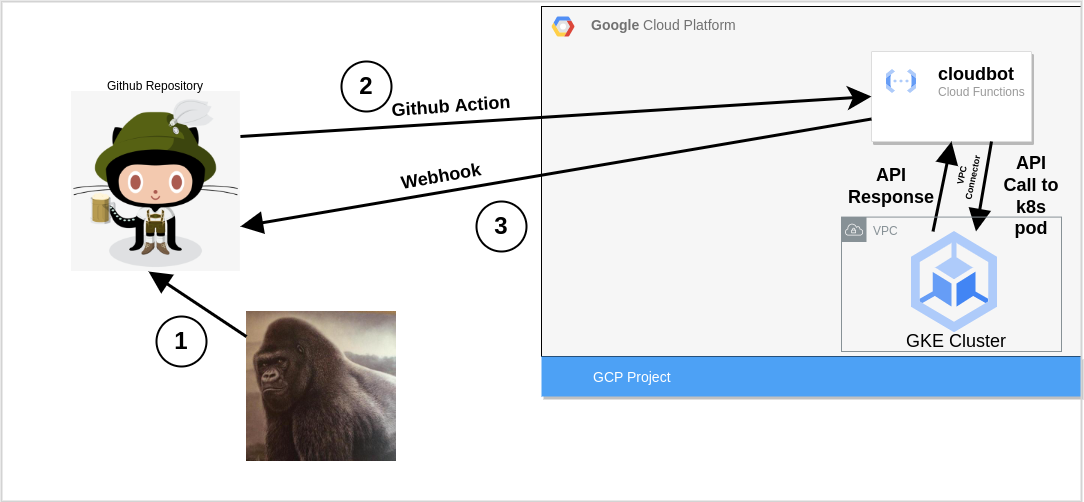
\includegraphics[width=0.785\textwidth]{../images/arch_diagrams-big-block.png}

\end{frame}

\begin{frame}
	\frametitle{Overview: Deployment}
	The big picture for deployment.
	\vspace{2mm}
\end{frame}

\begin{frame}
	\frametitle{Outline}
	A high level overview of the learning path is as follows:
	\begin{raggedright}
		\begin{itemize}
			\item Prerequisites
			\item Github setup.
			\item Set up a development environment.
			\item Review the Python source for the bot.
			\item Configure Terraform and deploy the bot.
			\item Test it out.
			\item Explore possibilities for extending the functionality.
		\end{itemize}
	\end{raggedright}
	\vspace{2mm}
\end{frame}

\begin{frame}
	\frametitle{Setup: VSCode}
	VSCode (\href{https://code.visualstudio.com}{https://code.visualstudio.com})
	\begin{itemize}
		\item Windows 64 bit User Installer: \href{https://prereqs.codemash.org/Files/VVSCodeUserSetup-x64-1.73.1.exe}{VSCodeUserSetup-x64-1.73.1.exe}
		\item Mac Universal: \href{https://prereqs.codemash.org/Files/VSCode-darwin-universal.zip}{VSCode-darwin-universal.zip}
		\item Linux (Debian, Ubuntu): \href{https://prereqs.codemash.org/Files/code_1.73.1-1667967334_amd64.deb}{code\_1.73.1-1667967334\_amd64.deb}
		\item  Linux (Red Hat, Fedora, SUSE): \href{https://prereqs.codemash.org/Files/code-1.73.1-1667967421.el7.x86_64.rpm}{code-1.73.1-1667967421.el7.x86\_64.rpm}
	\end{itemize}
\end{frame}

\begin{frame}
	\frametitle{Setup: git}
	GIT (\href{https://git-scm.com/downloads}{https://git-scm.com/downloads})
	\begin{itemize}
		\item Windows 32 Bit: \href{https://prereqs.codemash.org/Files/Git-2.38.1-64-bit.exe}{Git-2.38.1-64-bit.exe}
		\item Windows 64 Bit: \href{https://prereqs.codemash.org/Files/Git-2.38.1-32-bit.exe}{Git-2.38.1-32-bit.exe}
		\item Mac: \href{https://prereqs.codemash.org/Files/git-2.15.0-intel-universal-mavericks.dmg}{git-2.15.0-intel-universal-mavericks.dmg}
	\end{itemize}
\end{frame}

\begin{frame}
	\frametitle{Setup: Docker Desktop}
	Docker Desktop (\href{https://www.docker.com/}{https://www.docker.com/})

	\begin{itemize}
		\item Windows: \href{https://prereqs.codemash.org/Files/Docker\%20Desktop\%20Installer.exe}{Docker Desktop Installer.exe}
		\item MacOS (Intel Chip): \href{https://prereqs.codemash.org/Files/Docker.dmg}{Docker.dmg}
		\item MacOS (M1 Chip): \href{https://prereqs.codemash.org/Files/Chip/Docker.dmg}{Docker.dmg}
		\item Linux instructions can be found: \href{https://docs.docker.com/desktop/install/linux-install/}{here}
	\end{itemize}
\end{frame}

\begin{frame}
	\frametitle{Resources}
	\href{https://www.codemash.org/session-details/?id=375030}{Click here for Session Details}
	\vspace{2mm}

	Project source files are available: \url{https://github.com/devsecfranklin/workshop-codemash-2023}
	\vspace{2mm}

	Prerequisites are \href{https://prereqs.codemash.org/}{available at this link}.
\end{frame}

\begin{frame}
	\frametitle{Contact}
	\begin{columns}
		\begin{column}{0.5\textwidth}
			Mastodon: ``@devsecfranklin@defcon.social''
			\vspace{2mm}

			E-mail: \textbf{\href{mailto:devsecfranklin@duck.com}{devsecfranklin@duck.com}}
		\end{column}
		\begin{column}{0.5\textwidth}
			\begin{center}
				
\includegraphics[width=0.785\textwidth]{../images/rilla.jpg}
			\end{center}
		\end{column}
	\end{columns}
\end{frame}

\end{document}